\documentclass[a4paper,12pt,ngerman]{scrartcl}
\usepackage{babel}
\usepackage[T1]{fontenc}
\usepackage[utf8]{inputenc}
\usepackage{csquotes}
\MakeOuterQuote{"}
\usepackage[a4paper,left=4cm,right=2cm,top=2.5cm,bottom=2.5cm]{geometry}

\usepackage{amsmath}
\usepackage{amssymb}
\usepackage{amsthm}
\usepackage{nicefrac}

\usepackage[shortlabels]{enumitem}

\usepackage{graphicx}
\usepackage{subfig}
\usepackage{float}

\title{Die Heisenberg'sche Unschärferelation anhand von diskreten Wahrscheinlichkeitsverteilungen}
\author{Silas Alberti}
\date{Februar 2018}

\theoremstyle{plain}
\newtheorem{definition}{Definition}

\theoremstyle{plain}
\newtheorem{theorem}{Satz}

\theoremstyle{plain}
\newtheorem{postulate}{Postulat}

\theoremstyle{plain}
\newtheorem{corollary}{Korollar}

% Line spacing
\renewcommand{\baselinestretch}{1.5} 

\newcommand{\Z}{\mathbb{Z}}
\newcommand{\C}{\mathbb{C}}
\newcommand{\Cn}{\mathbb{C}_\mathbb{n}}
\newcommand{\T}{\mathbb{T}}
\newcommand{\X}{\mathbb{X}}
\newcommand{\N}{\mathbb{N}}

\newcommand{\at}[1]{\;\rtimes_{#1}\;}

\begin{document}

\maketitle

\tableofcontents

% Suppressing line numbering of first page
\thispagestyle{empty}
\clearpage
\setcounter{page}{1}

\section{Einleitung}

Dank der heutzutage weit fortgeschrittenen Displaytechnologie in Form von UHD-Auflösungen und 4K-Fernsehern vergisst man schon fast, dass auch die geradezu lebensecht darstellenden Monitore, das Bild dennoch aus einer Vielzahl an einzelnen Pixeln zusammensetzen. Dem entgegen stellt sich die sogenannte Pixel-Art, die gezielt niedrigere Auflösungen als Stilmittel verwendet. Dabei setzt der Pixel-Artist das Bild meist akribisch Pixel für Pixel zusammen ohne von den Vorteilen höherer Bearbeitungsebenen zu profitieren, die moderne Software bietet.

% Bild: Pixel-Art, z.B. Künstler-Grupp eBoy%

Sehr interessant sind die Einschränkungen, die diese Form der Bilderstellung dem Künstler schafft. So sind grundlegende geometrische Formen wie gerade Linien nur parallel zu den Linien des Rasters möglich. Erst recht problematisch wird es für komplexere Formen wie z.B. Kreise, die sich zwar mehr und mehr approximieren, aber tatsächlich nie perfekt umsetzen lassen. In der Pixel-Art-Szene wurde aus dem Streben nach der bestmöglichen Approximation von Kreisen, Linien und ähnlichem bereits eine eigene Wissenschaft.

% Bild: Kreis (oder Linien), ins Abbildungsverzeichnis? %

In der Realität außerhalb der Computer-Bildschirme hingegen -- so könnte man sich im Angesicht dieser Unvollkommenheit zureden -- existieren solche Probleme nicht; man könne ja unendlich weit "reinzoomen" in unser Universum. Derartige Überlegungen finden ihren Höhepunkt z.B. in der Analysis, genauer in der Infinitesimalrechnung, die mathematische Sachverhalte bis in unendliche Genauigkeit darstellen kann. 

Der elementare Gegensatz sind hier die mathematischen Begriffe \textit{diskret} und \textit{kontinuerlich}. Ein Computer-Bildschirm, der aus einer endlichen Anzahl an Pixeln besteht, kann nur diskretes fassen, während unser Universum (scheinbar) auch kontinuierliche Größen fassen kann. Mathematisch präziser formuliert, betrachtet die diskrete Mathematik nur endliche oder abzählbar unendliche Mengen, während die nicht-diskrete Mathematik (z.B. die Analysis) insbesondere eben auch überabzählbar unendliche Mengen wie die reellen Zahlen untersucht. So entstehen Konzepte wie die Stetigkeit einer Variable, die im Diskreten nicht existieren können.

Bereits gegen Ende des 19. Jh. stellte sich jedoch heraus, dass bisher für kontinuierlich gehaltene physikalische Größen und Phänomene wie die Ladung oder das Licht aus diskreten Grundeinheiten, sogenannten \textit{quanta} bestehen (d.h. Elektronen im Fall von Ladung; Photonen im Fall von Licht). Im Zuge dessen entwickelte sich Anfang des 20. Jh. die Quantenphysik, welche Phänomene und Größen, die nur feste diskrete Werte annehmen können, untersucht. Letzteres wird auch als \textit{Quantelung} bezeichnet.

Als Gründervater der Quantenphysik gilt der deutsche Physiker Max Planck (* 1858; \textdagger 1947), der erstmalig die Quantelung im Falle von Energie beschrieb. Nach ihm benannt ist auch die Planck-Länge
\[ l_P \approx 1.616 229 \cdot 10^{-35}m,\]
die der Anstoß für die in dieser Arbeit geführten Überlegungen ist. Der aktuellen -- noch nicht bewiesenen -- Theorie der Schleifenquantengravitation zufolge, die als die einzige weit entwickelte Alternative zur bekannteren String-Theorie gilt, ist nämlich das gesamte Universum durch die Planck-Länge quantisiert. Einfach dargestellt könnte man sagen, unser Universum bestehe aus Pixeln der Größe der Planck-Länge.

Wie in der Pixel-Art wäre es demnach tatsächlich nicht möglich, in unserem Universum einen perfekten Kreis zu erschaffen. 

Des Weiteren lässt sich die Planck-Zeit definieren
\[t_P \approx 5.39116\cdot 10^{-44}s,\]
die in der Schleifenquantengravitation die diskrete Grundeinheit der Zeit ist. Damit wäre sie im Kontext der eben bereits aufgefassten Computerbildschirm-Analogie mit der vergangenen Zeit zwischen zwei Frames z.B. eines digitalen Videos vergleichbar. 

Ohne Anspruch auf physikalische Treffsicherheit spielt diese Arbeit mit dem Konzept von diskreten Raum- und Zeiteinheiten unter der Annahme, dass die nicht unterschritten werden können. Wir werden grundlegende Teilchenbewegungen modellieren mit dem Ziel, herauszufinden, welche Implikationen diese Diskretheit birgt. 

Ich möchte nochmals betonen, dass ich keinesfalls behaupte, von den physikalischen Details auch nur annähernd Ahnung zu haben -- die tatsächliche moderne Quantenphysik ist wesentlich komplexer. Es handelt sich hierbei um rein mathematische Überlegungen, die keinen Zusammenhang zu echten physikalischen Phänomenen anstreben. Das Ziel ist es sich dem Konzept des Diskreten zu Nähern und herauszufinden, was für Folgen dies unter anderem haben könnte. % Erster und letzter Satz überarbeiten %

Im Laufe der Arbeit werde ich öfters Parallelen zu quantenphysikalischen Phänomenen ziehen, die eher als Anekdote zu sehen sind. %Ausführen%

\subsection{Die Heisenberg'sche Unschärferelation}

% Vorstellen %

\[\sigma_x \sigma_p \geq \frac{\hbar}{2}\]

\section{Hauptteil}

Begeben wir uns also auf die tiefstmögliche Ebene. Im Zentrum der folgenden Überlegungen wird ein "Teilchen" der Größe einer Planck-Länge stehen. Dabei sei der Begriff als ein reines mathematisches Objekt zu verstehen, ohne direkte physikalische Interpretation.

Im Folgenden werden wir die Konzepte \textit{Ort} und \textit{Zeit} benötigen. Bevor wir deren Struktur konkretisieren, betrachten wir sie erstmal als abstrakte Konzepte. Die folgenden Definitionen sind nicht ausreichend, um Bewegungen eines Teilchens eine vollständige Grundlage zu bieten; es fehlen Konzepte wie Distanz und Richtung. Dennoch wollen wir bereits eine Auffassung von Benachbarung im Raum und Aufeinanderfolgen in Zeit schaffen, da diese Zusammenhänge in unserem Modell das Konzept des "Abstandes" von Planck-Länge bzw. Planck-Zeit umsetzen.

\begin{definition}\label{def_ortundzeit}
\begin{enumerate}[(a)]
	\item Wir können eine Menge $\X$ als \textbf{diskreter Raum} 	bezeichnen, wenn sie maximal abzählbar unendlich ist, d.h. 			wenn
	\[ |\X| \leq \aleph_0,\]
	und außerdem eine \textbf{Nachbarschaftsfunktion} $\delta: 			\X^2\rightarrow\{0,1\}$ existiert mit
	\begin{enumerate}[(i)]
		\item$\forall\, x\in\X\quad\exists\, x_0\in\X: \quad				\delta(x,x_0)=1,$
		\item$\forall\, x_0,x_1\in\X: \quad\delta(x_0,x_1)=					\delta(x_1,x_0),$ 
		\item$\forall\, x\in\X: \quad \delta(x,x)=0.$
	\end{enumerate}
	Ein $x\in\X$ bezeichnen wir als \textbf{Position}. Wenn für 		$x_0,x_1\in\X$ gilt, dass $\delta(x_0,x_1)=1$ bezeichnen wir 	sie als \textbf{benachbart}, andernfalls als \textbf{nicht 			benachbart}. 
	\item Wir können eine Menge $\T$ als \textbf{diskrete Zeit} 		bezeichnen, wenn sie maximal abzählbar unendlich ist, d.h. 			wenn
	\[ |\T| \leq \aleph_0,\]
	und außerdem eine \textbf{Nachfolgerfunktion} $\mu: \T 				\rightarrow \T$ existiert, wobei $\forall \,t\in\T: \;\mu(t)		\neq t$. Ein $t\in\T$ bezeichnen wir als \textbf{Zeitpunkt}.
\end{enumerate}
\end{definition} %Geordnetheit, etc. %

So wird $\X$ in der Praxis z.B. ein durch ganzzahlige, kartesische Koordinaten beschreibbarer euklidischer Raum\footnote{In der Realität ist der Raum wahrscheinlich nicht euklidisch (vgl. Raumkrümmung in der Relativitätstheorie).} sein. Die Zeit $\T$ werden wir im Laufe dieser Arbeit durch die ganzen Zahlen umsetzen, wobei $\mu(t):=t+1$ sei.

%Woanders noch verwenden:%
%Dass die Voraussetzungen von Definition \ref{def_ortundzeit} (b) dabei erfüllt sind, ist straightforward ($\rightarrow$ Anhang 4.1 \textit{Straightforwardness von Beweisen}).%

% Definition von Teilchen selbst?%

\begin{definition}
Es sei $\Phi$ ein \textbf{Teilchen}. Des Weiteren bezeichne $x\in\X$ eine Position und $t\in\T$ einen Zeitpunkt. Wir sagen
\[\Phi \at{t} x,\]
wenn sich $\Phi$ an der Position $x$ zum Zeitpunkt $t$ befindet.
\end{definition}

\subsection{Grundprinzipien}

Benachbarte Punkte sind Punkte im Abstand einer Planck-Länge. %Anders formulieren%
Der Nachfolger eines Zeitpunkts, ist ein Zeitpunkt in einer Planck-Zeit Abstand. Interessanterweise gilt
\[c=\frac{l_P}{t_P},\]
wobei $c$ die Lichtgeschwindigkeit ist. Die in der Physik gemeinhin akzeptierte Annahme, dass die Lichtgeschwindigkeit nicht überschritten werden kann, übersetzen wir mit Postulat \ref{pos_lightspeed} in unser mathematisches Modell.

\begin{postulate}\label{pos_lightspeed}
Es sei $\Phi$ ein Teilchen. Des Weiteren gelte für ein $x_0\in\X$ und ein $t\in\T$
\[\Phi \at{t} x_0.\]
Wenn für ein $x_1\in\X$ 
\[\Phi \at{\mu(t)} x_1\]
gilt, dann muss $\delta(x_0,x_1)=1$ oder $x_0=x_1$ gelten.
\end{postulate}

Dieses Geschwindigkeitslimit bezeichnen wir im Folgenden als \textit{Maximalgeschwindigkeit}, um nicht das Wort Lichtgeschwindigkeit verwenden zu müssen.

\subsection{Eindimensionale Bewegungen}

Im eindimensionalen Fall können wir den Raum durch die ganze Zahlen darstellen, d.h. $\X := \Z$. Die Nachbarschaftsfunktion $\delta$ ist in diesem Fall definiert durch 
\[\delta(x_0,x_1):=\begin{cases}
1 \quad&\mbox{wenn } |x_0-x_1|=1,\\
0 \quad&\mbox{ansonsten.}
\end{cases}\]

Betrachten wir also ein Teilchen $\Phi$, für das $\Phi \at{0} 0$ gelte. Stellen wir uns $\Phi$ zum Zeitpunkt 0 an der Stelle 0 einer horizontalen Zahlengeraden vor mit den positiven Zahlen zur Rechten. Eine Bewegung von $\Phi$ mit Maximalgeschwindigkeit nach rechts, ließe sich nun folgendermaßen beschreiben:
\[\Phi \at{0} 0,\quad \Phi \at{1} 1,\quad \Phi \at{2} 2,\quad\Phi\at{3} 3,\;\dots\]

Was ist allerdings, wenn $\Phi$ sich langsamer bewegt? Mal angenommen, es bewegte sich in halber Maximalgeschwindigkeit: Da es sich in einem Zeitschritt um entweder genau eine Einheit oder gar keine bewegen muss, ist es nicht möglich innerhalb einer Zeiteinheit eine halbe Maximalgeschwindigkeit umzusetzen. 

Wenn sich $\Phi$ allerdings in zwei Zeiteinheiten um insgesamt eine Raumeinheit bewegt, dann ist die effektive Geschwindigkeit tatsächlich die halbe Maximalgeschwindigkeit. Ähnlich wie also Pixel-Artists gerade Linien oder Kreise approximieren, so können wir Bewegungen auf anderen Geschwindigkeiten als der Maximalgeschwindigkeit approximieren durch abwechselndes Verweilen und Bewegen auf Maximalgeschwindigkeit.

%Abbildung Linie von Pixel-Artist und Bewegung%

Es gibt zwei Arten, eine Bewegung auf halber Geschwindigkeit in den ersten beiden Zeitschritten zu vollziehen:
\[\Phi\at{0}0,\;\Phi\at{1}0,\; \Phi\at{2}1 \quad\text{und}\quad \Phi\at{0}0,\;\Phi\at{1}1,\;\Phi\at{2}1.\]

Wie entscheidet sich also, wo sich $\Phi$ zum Zeitpunkt 1 befindet? Da beide gerade aufgezeigten Varianten -- aus unserem Blickwinkel -- vollkommen gleichwertig sind, müssten wir, um ein deterministisches Gesetz für die Bewegung von $\Phi$ zu haben, arbiträr eine der beiden Varianten bevorzugen. Wenn wir dies nicht tun wollen, bleibt es uns nur übrig, die Voraussetzung des Determinismus aufzugeben -- genau wie es die Quantenphysik auch tat. 

So sagen wir nun also: Mit einer Wahrscheinlichkeit von $\frac{1}{2}$ befindet sich $\Phi$ zum Zeitpunkt 1 an Position 0 und mit einer Wahrscheinlichkeit von $\frac{1}{2}$ befindet es sich an Position 1 zu diesem Zeitpunkt. In anderen Worten: 
\[P(\Phi\at{1}0)=\frac{1}{2} \quad\text{und}\quad P(\Phi\at{1}1)=\frac{1}{2}.\]

Im Folgenden werden wir uns allerdings gar nicht dafür interessieren, an welcher Position sich $\Phi$ zum Zeitpunkt 1 letztlich befinden wird; uns interessiert lediglich mit welcher Wahrscheinlichkeit es sich wo befindet. Eine Interpretation der Quantemechanik besagt, dass für bestimmte Objekte mit probabilistischen Eigenschaften -- ähnlich zu denen unseres Teilchens -- sich ohne "Messung" gar nicht erst entscheidet, welche der verschiedenen möglichen Eigenschaften das betrachte Objekt tatsächlich einnimmt; es befindet sich in einer \textit{Superposition} aus den verschiedenen Möglichkeiten. Genauso können wir sagen, dass $\Phi$ zum Zeiptunkt 1 in einer Superposition der Positionen 0 und 1 ist.

\begin{definition}\label{def_psi}
Die Position eines Teilchen $\Phi$ sei vollständig charakterisiert durch eine Charakterisierungsfunktion $\psi: \X\times\T \rightarrow [0;1]$ mit
\[\forall\, x\in\X\quad\forall\, t\in\T:\quad
P(\Phi\at{t}x)=\psi(x,t).\]
\end{definition}

\begin{corollary}\label{cor_summe}
Da es sich bei gegebenem $t$ bei $\psi$ um eine Wahrscheinlichkeitsverteilung in $x$ handelt, gilt
\[\sum_{x\in\X} \psi(x,t)=1 \quad\forall\,t\in\T.\]
\end{corollary}

Aufgrund von Korollar \ref{cor_summe} betrachten wir von nun an bei einem gegebenen Zeitpunkt $t_0$ nur noch die Werte von $\psi$ mit $\psi(x,t_0)\neq0$. Alle anderen Werte seien dann implizit 0.

Wir wissen also, dass bei einer Geschwindigkeit von $\frac{1}{2}$  eben $\psi(0,0)=1$, $\psi(0,1)=\frac{1}{2}$ und $\psi(1,1)=\frac{1}{2}$ gilt. Zum Zeitpunkt 2 sollte nun erwartungsgemäß $\psi(0,2)=0$ und $\psi(1,2)=1$ gelten, womit sich $\Phi$ in zwei Zeiteinheiten um eine Längeneinheit bewegt hat. Wir erinnern uns allerdings daran, dass wir durch $\psi$ nur die Superpositionen verschiedener einzelner Bewegungen simulieren. Im Falle von $\Phi\at{1}0$ bewegt sich $\Phi$ also zum Zeitpunkt 2 um eine Einheit weiter; bei $\Phi\at{1}1$ bleibt es hingegen stehen. Die Gesetzesmäßigkeiten für die Fortbewegung von $\Phi$ unterscheiden sich hier also in beiden Fällen. Eine Grundvoraussetzung sei es allerdings, dass wir eindeutige Gesetze haben, die für alle Positionen und Zeitpunkte gleichermaßen gelten.

Dieses Problem könnte durch eine weitere Variable gelöst werden, die zum Zeitpunkt 1 variiert wird, je nach dem, ob sich bewegt wurde oder nicht. Diese könnte dann für den Zeitpunkt 2 zur Entscheidung zwischen Bewegen und Nichtbewegen genutzt werden. Wir entscheiden uns jedoch bewusst gegen eine solche Variable und betrachten dagegen die Folgerungen, die der Verzicht auf eine solche bietet.

\begin{postulate}\label{pos_einstein}
Es sei $\psi$ eine Charakterisierungsfunktion, für die beliebige Gesetzesmäßigkeiten gelten. Dann gelte für alle Charakterisierungsfunktionen $\psi_0$ und $\psi_1$ dieselben Gesetzesmäßigkeiten insofern sie
\[\psi(x,t)=a\cdot\psi_0(x,t)+b\cdot\psi_1(x,t)\quad\forall\,x\in\X\;\;\forall\,t \in\T\]
mit $a,b\in[0,1]$ und $a+b=1$ erfüllen.
\end{postulate}

Wir können also unsere Funktion $\psi$ in $\psi_0$ mit $\psi_0(0,1)=1$ und $\psi_1$ mit $\psi_1(1,1)=1$ für $a=b=\frac{1}{2}$ aufteilen. Es gilt unter Anwendung derselben Gesetzesmäßigkeiten, wie wir bei $\psi$ verwendeten, für $\psi_0$, dass $\psi_0(0,2)=\frac{1}{2}$ und $\psi_0(1,2)=\frac{1}{2}$ und für $\psi_1$, dass $\psi_1(1,2)=\frac{1}{2}$ und $\psi_1(2,2)=\frac{1}{2}$. 

Durch das gewichtete Summieren erhalten wir wiederum für $\psi$, dass $\psi(0,2)=\frac{1}{4}$, $\psi(1,2)=\frac{1}{2}$ und $\psi(2,2)=\frac{1}{4}$. Der Erwartungswert der Position von $\Phi$ ist also immer noch bei $x=1$; nur die Varianz hat sich durch Postulat \ref{pos_einstein} vergrößert.

Mittels mehrfachen Anwendens von Postulat \ref{pos_einstein} kann man $\psi$ auch für die Zeitpunkte $t>2$ bestimmen. Man wird erkennen, dass es sich bei $\psi$ bei gegebenem $t$ um eine Binomialverteilung mit Erwartungswert bei $x=\frac{1}{2}t$ handelt. Während sich also die Varianz von $\psi$ immer weiter erhöht, bewegt sich der Erwartungswert exakt mit der Geschwindigkeit $\frac{1}{2}$.

\subsubsection{Allgemeine Geschwindigkeit}

Für eine Geschwindigkeit $v$ eines Teilchens muss gelten $|v|\leq 1$. Eine negative Geschwindigkeit könnte in diesem Kontext als Bewegung in negative x-Richtung aufgefasst werden, allerdings beschränken wir uns der Einfachheit auf den positiven Fall. Der negative Fall würde analog, nur mit anderen Vorzeichen, funktionieren, und eine Beachtung dessen würde die Komplexität der Gleichungen, nicht aber nicht die anzustrebende Einsicht erhöhen.

Naheliegend ist nun die Gesetzesmäßigkeit, dass bei gegebenem $v\geq0$, $x_0$ und $t_0$ mit $\psi(x_0,t_0)=1$ gilt, dass $\psi(x_0,t_0+1)=1-v$ und $\psi(x_0+1,t_0+1)=v$. So befindet sich der Erwartungswerten von $\psi$ für $t=t_0+1$ bei $x=x_0+v$. Innerhalb einer Zeiteinheit hat sich das Teilchen durchschnittlich also um $v$ bewegt. 

Durch mehrfache Anwendung von Postulat \ref{pos_einstein} erhält man die Rekursionsgleichung
\[\psi(x,t)=v\cdot\psi(x-1,t-1)+(1-v)\cdot\psi(x,t-1) \quad\forall\, t>t_0 \;\;\forall x\in\X.\]

Es lässt sich leicht beweisen, dass der Erwartungswert von $\psi$ zum Zeitpunkt $t=t_0+\Delta t$ genau $x=x_0+v\cdot\Delta t$ ist. Durch diese Rekursionsgleichung ist also die Bewegung im eindimensionalen Fall vollständig beschrieben, weswegen wir uns nun der zweiten Dimension zuwenden.

%In Abhängigkeit einer Startposition $\Phi\at{t_0}x_0$ und einer Geschwindigkeit $v$ die Funktion $\psi$ durch folgende Rekursionsgleichung charakterisieren:
%\begin{enumerate}
%\item $\psi(x_0,t_0)=1$
%\item $\psi(x,t_0)=0 \quad\forall\, x\in\Z$
%\item $\psi(x,t)=v\cdot\psi(x-1,t-1)\\\phantom{\psi(x,t)=}+(1-v)\cdot\psi(x,t-1) \quad\forall\, t>t_0 \;\;\forall x\in\X$
%\end{enumerate}


\subsection{Zweidimensionale Bewegungen}

Ein zweidimensionaler, diskreter Raum könnte zum Beispiel durch $\X=\Z^2$ dargestellt werden. Ähnlich wie wir es im eindimensionalen Fall hatten, beschränken wir uns in dieser Arbeit der Übersichtlichkeit halber allerdings auf den 1. Quadranten, d.h. beide Komponenten einer Position seien positiv. 

Es sei also $\X=\N^2$ und $\T=\Z$. Neben der Geschwindigkeit $v\in[0;1]$ muss nun für die Bewegung eines Teilchens ebenfalls eine Richtung $\theta\in[0;\nicefrac{\tau}{4}]$ mit $\tau=2\pi$ gegeben sein.

Betrachten wir nun zuerst den Fall $\theta=\nicefrac{\tau}{8}\;\widehat{=}\;45^{\,\circ}$. Außerdem gelte $\Phi\at{0} (0,0)$. Zum Zeitpunkt 1 kann $\Phi$ sich aufgrund unserer Grundvoraussetzung der maximalen Bewegung um eine Längeneinheit pro Zeitschritt nicht auf Position $(1,1)$ befinden, was der geringsten, eindeutigen Bewegung im $45^{\,\circ}$-Winkel entspräche.

Bei einer Bewegung mit maximaler Geschwindigkeit befände sich $\Phi$ zum Zeitpunkt 1 in einer Superposition aus $(0,1)$ und $(1,0)$. Es gilt also $\psi((1,0),1)=\frac{1}{2}$ und $\psi((0,1),1)=\frac{1}{2}$.

Für ein allgemeines $\theta\in[0;\nicefrac{\tau}{4}]$ können wir sagen $\psi((1,0),1)=\frac{\sin(\theta)}{\sin(\theta)+\cos(\theta)}$ und $\psi((1,0),1)=\frac{\cos(\theta)}{\sin(\theta)+\cos(\theta)}$. Der Erwartungswert der Position zum Zeitpunkt 1 ist damit 
$\left(\frac{\sin(\theta)}{\sin(\theta)+\cos(\theta)},\frac{\cos(\theta)}{\sin(\theta)+\cos(\theta)}\right)$. Der Winkel zur x-Achse ist also tatsächlich $\theta$. 

Geschwindigkeit können wir nun noch umsetzen, indem wir -- analog zum eindimensionalen Fall -- eine Bewegung der Geschwindigkeit $v$ als Superposition aus der Situation mit gar keiner Bewegung und der Situation mit der, eben schon formulierten, maximalen Bewegung darstellen, gewichtet jeweils mit $1-v$ bzw. $v$. So erhalten wir $\psi((0,0),1)=1-v$,\; $\psi((1,0),1)=\frac{v\cdot\sin(\theta)}{\sin(\theta)+\cos(\theta)}$ und $\psi((1,0),1)=\frac{v\cdot\cos(\theta)}{\sin(\theta)+\cos(\theta)}$. Als Betrag des Erwartungswertes erhalten wir dann
\begin{align*}
&\sqrt{\left(\frac{v\cdot\sin(\theta)}{\sin(\theta)+\cos(\theta)}\right)^2+\left(\frac{v\cdot\cos(\theta)}{\sin(\theta)+\cos(\theta)}\right)^2}\\
=&\;\sqrt{\frac{v^2(\sin^2(\theta)+\cos^2(\theta))}{(\sin(\theta)+\cos(\theta))^2}}=\frac{v}{\sin(\theta)+\cos(\theta)}.
\end{align*}
Wir wollen allerdings Geschwindigkeiten nicht derart charakterisieren, dass die dann tatsächlich zurückgelegte Distanz -- am Betrag des Erwartungswerts gemessen -- zusätzlich noch von $\theta$ abhängt, da dies mit der Auffassung von Bewegungen in der Realität nicht übereinstimmt. Daher charakterisieren wir unser Teilchen durch die 
Erwartungswertgeschwindigkeit $v_e:=\frac{v}{\sin(\theta)+\cos(\theta)}.$ 

Wegen $v\leq1$, erhalten wir $v_e\leq\frac{1}{\sin(\theta)+\cos(\theta)}$. Der Nenner auf der rechten Seite wird maximal für $\theta=\nicefrac{\tau}{8}$, wie sich durch Ableiten feststellen lässt. Da wir ein $v_e$ unabhängig von $\theta$ wählen können wollen, muss 
\[v_e\leq\frac{1}{\sin\left(\frac{\tau}{8}\right)+\cos\left(\frac{\tau}{8}\right)}=\frac{1}{\sqrt{2}}\]
gelten, um $v\leq1$ zu garantieren. Interessanterweise erhalten wir also im zweidimensionalen Fall eine niedrigeres Geschwindigkeitslimit, wenn wir den Erwartungswert eines Teilchens als die Maßgabe für eine Geschwindigkeitsdefinition wählen. 

Es sei $\pmb{i}=(1,0)$ und $\pmb{j}=(0,1)$. Wir charakterisieren ein Teilchen $\Phi$ mit beliebigem $v_e\in[0;\frac{1}{\sqrt{2}}]$ und $\theta\in[0;\nicefrac{\tau}{4}]$, so erhalten wir für die Charakterisierungsfunktion mit $\psi((x_0,t_0)=1$ für beliebige $x_0\in\N^2$, $t_0\in\Z$, dass 
\begin{itemize}
\item $\psi(x_0,\;t_0+1)=1-v_e(\sin(\theta+\cos(\theta))$,
\item $\psi(x_0-\pmb{i},\;t_0+1)=v_e\cdot\sin(\theta)$,
\item $\psi(x_0-\pmb{j},\;1t_0+1)=v_e\cdot\cos(\theta)$.
\end{itemize}
Dadurch sowie durch Anwendung von Postulat \ref{pos_einstein} auf eine allgemeine Charakterisierungsfunktion $\psi$ erhalten wir also die Rekursionsgleichung
\begin{align*}
\begin{split}
\psi(x,\,t)=\phantom{+}&\psi(x,\;t-1)\cdot(1-v_e(\sin(\theta+\cos(\theta)))\\
+\,&\psi(x-\pmb{i},\;t-1)\cdot(v_e\cdot\sin(\theta))\\
+\,&\psi(x-\pmb{j},\;t-1)\cdot(v_e\cdot\sin(\theta)).
\end{split} \forall\;x\in\N^2,\,t\in\Z
\end{align*}
Damit haben wir die Bewegung von einem $\Phi$ im ersten Quadranten des zweidimensionalen Raums vollständig charakterisiert. Simulationen derartiger Bewegungen befinden sich als Bilderserien im Anhang und können auch im Internet als Animationen abgerufen werden (für weiteres siehe Anhang).

\subsection{Erweiterung des Modells}

\subsubsection{Problematik}

Betrachten wir für ein beliebiges $t\in\Z$ die Varianz der Position
\[\sigma_x^2:=\sum_{x\in\N^2}|x-\mu_x|^2\cdot\psi(x,t)\]
mit dem Erwartungswert $\mu_x=\sum_{x\in\N^2}x\cdot\psi(x,t)$. Wir wollen nun die Entwicklung von $\sigma_x^2$ über die Zeit $t$ unter der Startbedingung $\Phi\at{0}(0,0)$ untersuchen. In Abbildung \ref{fig_variance_time} sehen wir dies für verschiedene $\theta$ bei (a) für ein konstantes $v_e=\frac{1}{\sqrt{2}}$ und bei (b) für ein konstantes $v=1$.

In beiden Fällen sehen wir, dass die Varianz über die Zeit linear ansteigt. Vielmehr stellen wir fest, dass die Steigung der Varianz von $\theta$ abhängt. Bei dem konstantem $v$ schwankt sie zwischen 0 und $\frac{1}{2}$; bei dem konstantem $v_e$ schwankt sie zwischen ca. $0,207$ und $\frac{1}{2}$. Die verschiedenen Steigungen in Abhängigkeit von $\theta$ sind auch noch mal deutlich in Abbildung \ref{fig_variance_angle} gegenübergestellt.

Die Varianz sollte sich optimalerweise unabhängig von $\theta$ entwickeln -- bestenfalls wäre die Kurve in Abbildung \ref{fig_variance_angle} also eine horizontale Gerade. Dies ist jedoch nicht der Fall. Durch die Einführung von $v_e$ anstelle von $v$ haben wir den Einfluss von $\theta$ auf die Änderungsrate von $\sigma_x^2$ bereits reduziert, was die Sinnvollkeit dieser Entscheidung nur erneut bestätigt. 

Dennoch wäre das Modell treffender, wenn $\theta$ auf die Entwicklung der Varianz keinen Einfluss hätte, da sich andernfalls in einer derartig konstruierten Welt ein zugrundeliegendes Koordinatensystem feststellen lassen würde, wie es in unserem Universum nicht der Fall ist.

\subsubsection{Neudefinition}

Die im Laufe der Bewegung nicht eindeutig definierte Position, lässt sich auch als \textit{Unschärfe} in der Position bezeichnen. In der Quantenphysik tritt dieses Phänomen auch für die Geschwindigkeit\footnote{genau gesagt für den Impuls; da wir jedoch keine Massen betrachten, können wir den Impuls auf die Geschwindigkeit reduzieren} auf. Letzteres stellen wir in unserem Modell im Gegensatz zur Positionsunschärfe noch nicht fest. Die Geschwindigkeit ist als externe Größe bisher eindeutig gegeben gewesen.

Wir erweitern nun unsere Auffassung einer Charakterisierungsfunktion, so dass wir keine weiteren, externen Variablen mehr außer ihr benötigen.

\begin{postulate}
Der Zustand eines Teilchens $\Phi$ zum Zeitpunkt $t$ ist vollständig gegeben durch eine Charakterisierungsfunktion $\Psi: \X\times\T\rightarrow\C$ mit
\[\forall\, x\in\X\quad\forall\, t\in\T:\quad
P(\Phi\at{t}x)=|\Psi(x,t)|^2.\]
\end{postulate}

Dieser Schritt ist auch der Grund, warum Definition \ref{def_psi} von mir nicht als Postulat eingestuft wurde. Durch Setzen von $\psi(x,t):=|\Psi(x,t)|^2$ ist jene außerdem immer noch gültig, da ausdrücklich nur die Position charakterisiert wird.

Der Wertebereich der Charakterisierungsfunktion umfasst nun also die komplexen Zahlen. Neben des Betrags eines Funktionswertes von $\Psi$, die wie bereits zuvor die Positionswahrscheinlichkeiten repräsentiert, können nun zusätzlich durch das jeweilige komplexe Argument die ehemaligen Größen $\theta$ und $v_e$ kodiert werden.

Wie erhalten wir die Geschwindigkeit eines Teilchens $\Phi$ aus $\Psi$? In der Quantenphysik wie auch hier geschieht das durch eine \textit{Fourier-Transformation}. Typischerweise bezeichnet dies die Zerlegung eines Signals in der Zeitdomäne in seine Frequenzanteile. In unserem Sinne jedoch zerlegen wir ein Signal in der räumlichen Domäne in \glqq räumliche Frequenzen\grqq. Diese Überlegung und insbesondere der Zusammenhang dieser Frequenzzerlegung mit der Geschwindigkeit ist der einzig schwierig zu hinterfragende Schritt an unserer Konstruktion (für genaueres siehe 2.5).

Die übliche kontinuierliche Fourier-Transformation (FT) ist in unserem Fall aber nicht anwendbar. Das naheliegendste Pendant, die \textit{diskrete Fourier-Transformation (DFT)}, eignet sich auch nicht wegen ihrer Beschränkung auf endliche Definitionsbereiche. Stattdessen verwenden wir die \textit{zeitdiskrete Fourier-Transformation (DTFT)}, die als Grenzwert der DFT entsteht und sich für abzählbar unendliche Sachverhalte wie den unseren eignet. Als DTFT von $\Psi$ erhalten wir (Herleitung siehe %noch einfügen%) 
\[\widehat{\Psi}(\pmb{\omega},t) = \sum_{\pmb{x}\in\mathbb{N}^2}\Psi(\pmb{x},t)e^{-i\sqrt{2}\tau(\pmb{\omega}\cdot\pmb{x})}\]
mit $\pmb{x}\in\X=\N^2$,\; $\pmb{\omega}\in[0;\nicefrac{1}{\sqrt{2}}]\times[0;\nicefrac{1}{\sqrt{2}}]$ und $\pmb{\omega}\cdot\pmb{x}$ als Skalarprodukt, wobei $|\pmb{\omega}|\;\widehat{=}\;v$ und der Winkel von $\pmb{\omega}$ zur x-Achse $\theta$ entspräche.

Unsere Rekursionsgleichung lässt sich nun für $\X:=\N^2$ folgendermaßen aufstellen:
\begin{align*}
\Psi(\pmb{x},t) = \int_0^{\frac{1}{\sqrt2}}\int_0^{\frac{1}{\sqrt2}} 
\widehat{\Psi}(\pmb{\omega},t)
&\left[
\pmb{\omega}\cdot\left(\Psi(\pmb{x}-\hat{i},t-1),\Psi(\pmb{x}-\hat{j},t-1)\right)
\right.\\
&\left.\;+\;(1-|\pmb{\omega}|)\Psi(\pmb{x},t-1)\vphantom{\hat{\Psi}}\right]
\operatorname{d}\pmb{\omega}. 
\end{align*}

Löst dies unser Problem aus 2.4? Das kann nicht unmittelbar beurteilt werden: Einerseits haben wir somit keine externe Variable $\theta$, die die Varianz verändert auf eine Weise, wie sie unserer alltäglichen Vorstellung von einem relativistischen Raum widerspricht. Andererseits können wir hinterfragen, ob nicht vielleicht trotzdem eine Korrelation zwischen dem \textit{effektivem} $\theta$, d.h. dem, dass sich aus der DTFT ergibt, und der Varianz auftritt. Nicht zuletzt ist es fraglich, ob in einem diskreten Raum überhaupt die Möglichkeit "gleichwertiger Koordinatensysteme" unter Drehungen abseits von $90^{\,\circ}$-Schritten, d.h. Relativismus, realisierbar ist. 

\subsection{Die Unschärferelation}

Unschärfe tritt in diesem erweiterten Modell also nicht nur für die Position, sondern auch für die Geschwindigkeit auf. Durch den Zusammenhang von $\Psi$ und $\widehat{Psi}$ über die FT, gilt für sie mathematisch ganz natürlich, dass Unschärfeprinzip. Die Varianz beider Größen kann nicht gleichzeitig beliebig klein werden. 

Dies ist keine zufällige Eigenschaft der Natur, sondern eine inhärente Eigenschaft der FT. Ein Beweis dessen befindet sich in Anhang <noch einfügen>. Der einzige physikalische, d.h in gewissem Sinne überraschende Aspekt ist tatsächlich, dass $\Psi$ und $\widehat{\Psi}$, also Position und Geschwindigkeit (bzw. genauer: Impuls), eben durch die FT zusammenhängen.

Den Zusammenhang zwischen der Materiewelle eines Teilchens, d.h. der FT der Position, und dessen Impuls wurde 1924 erstmals von Louis de Broglie postuliert. Auf meiner Suche nach der Begründung für diesen Zusammenhang fand ich größtenteils Erklärungen, die sich darauf runterbrechen ließen, dass es sich dabei, um einen axiomatischen Sachverhalt handele. Ähnlich wie z.B. für die Newton'schen Axiome gebe es keine Möglichkeit eines Beweises; der Unterschied sei nur, dass wir für die Newton'sche Physik ein Intuition haben, da dessen Effekte unseren Gehirn im Laufe der Evolution zum Alltag wurden, während derartige quantenphysikalische Probleme für unsere Gehirne intuitiv nicht verständlich gemacht werden könnten.

Nicht zufriedengestellt 

\section{Perspektive}



\section{Anhang}

%\subsection{Straightforwardness von Beweisen}
%
%Im Laufe der Arbeit wird mehrmals das englische Wort "straightforward" verwendet, um die Auslassung von Beweisen zu begründen. Grob übersetzt bedeutet das Wort "trivial" oder auch "geradlinig durchführbar". Da ich das englische Wort als so treffend, jedwede deutsche Übersetzung jedoch für unpassend empfand, habe ich es wörtlich verwendet. Hier werde ich kurz erläutern, warum und in genau welchen Fällen ich mich dafür entschieden habe Beweise auszulassen.
%
%Als \textit{straightforward} bezeichne ich Beweise deren Herausforderung -- wenn sie nicht sowieso trivial sind -- nicht wie häufig in dem Finden einer kreativen bis zu genialen Idee liegt, sondern stattdessen in der Komplexität der Notation. Mathematische Notation ist stets nur der Annäherungsversuch an natürliche bzw. zugrundeliegende Wahrheiten oder Gesetzmäßigkeiten, die schwierig zu fassen sind. Manchmal wirken daher Zusammenhänge durch die Verschleierung der Notation als nicht-trivial, obwohl sie aus anderen Blickwinkeln betrachtet naheliegend bis zu offensichtlich sind. Beispielhaft lässt sich die Kettenregel in der Analysis nennen, die in Differentialquotienten (Leibniz-Notation) dargestellt naheliegend scheint,
%\[ \frac{\mathrm{d}y}{dx}\frac{dx}{dz} = \frac{dy}{dz},\]
%in der Lagrange-Notation dagegen nicht,
%\[ (f\circ g)'(x) = f'(g(x))g'(x). \]
%Des Weiteren ist der formale Beweis der Kettenregel mittels der h-Methode wesentlich komplizierter als das intuitive Verständnis des zugrundeliegenden Zusammenhangs, ohne jedoch weitere wesentliche Erkenntnis für letzteres zu bieten. Ich möchte nicht behaupten, dass ein genaues Studium diese Beweises überhaupt keine Erkenntnis bieten kann, sondern nur, dass diese Erkenntnis sehr verschlüsselt ist und durch ein anderes Medium wahrscheinlich besser vermittelt werden kann.
%
%Keinesfalls möchte ich die Wichtigkeit von Beweisen per se bestreiten und, um mit gutem Gewissen die Wahrheit der in der Arbeit behandelten Sachverhalte behaupten zu können, habe ich jeden der nicht angeführten Beweise selbst ausgearbeitet. Das ist wichtig, denn oft fallen einem im Beweisprozess Ausnahmen und Einschränkungen der zu zeigenden Aussage auf, die man vorher unter Umständen übersehen hatte. Für wahrhaftige Vollständigkeit müsste wohl jeder der ausgelassenen Beweise elaboriert werden, damit unter voller mathematischer Strenge von der Wahrheit der zu beweisenden Aussagen ausgegangen werden kann. 
%
%In dieser Arbeit ist dies jedoch nicht das Ziel; stattdessen soll sie dem Leser einen direkteren Mehrwert bieten. Technische Termumformungen u.ä. ohne signifikante Erkenntnis beim erstmaligen Betrachten stören lediglich den Lesefluss sowie die Dichte von relevanter Information in der Arbeit -- mit hoher Wahrscheinlichkeit würden sie in den meisten Fällen sowieso übersprungen werden. Nicht zuletzt auch noch wegen der Längenbeschränkung auf 12 Seiten, habe ich mich daher dazu entschlossen, diejenigen Beweise, die -- in meinen Augen -- straightforward sind, auszulassen.



\subsection{Abbildungen}

\begin{figure}[h]%
    \centering
    \subfloat[Für konstantes $v_e$]{{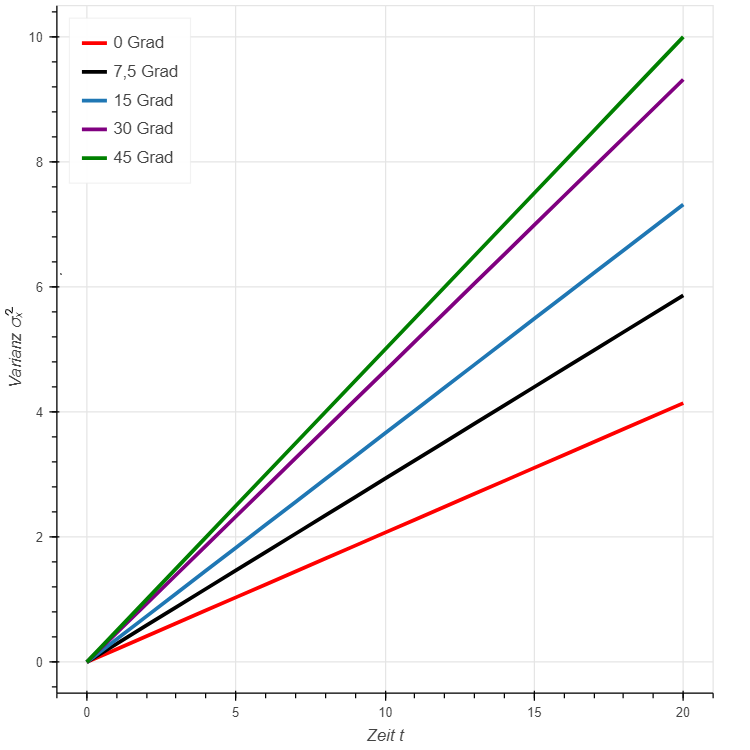
\includegraphics[width=6.5cm]{varianz-zeit_konstantes_v_e.png} }}%
    \qquad
    \subfloat[Für konstantes $v$]{{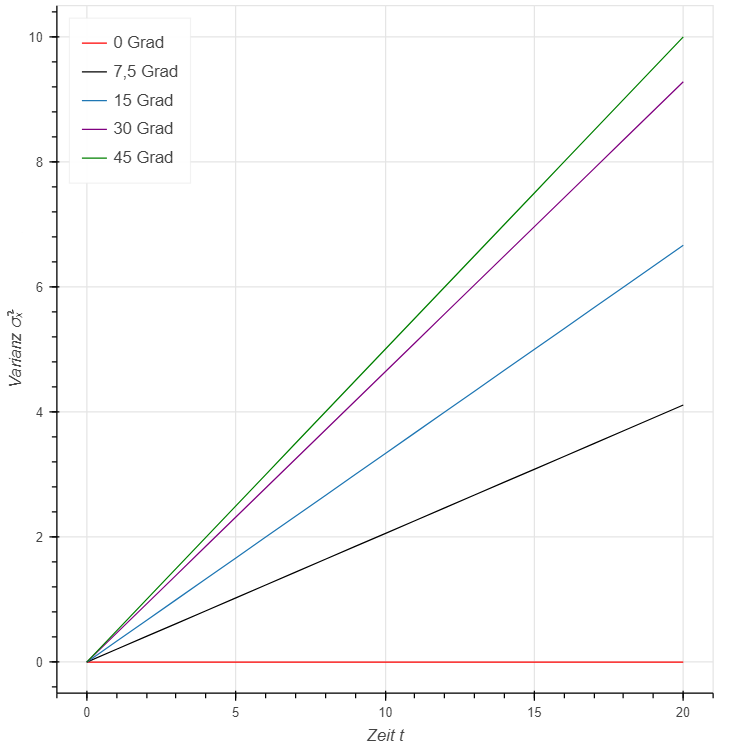
\includegraphics[width=6.5cm]{varianz-zeit_konstantes_v.png} }}%
    \caption{Varianz $\sigma_x$ im Verlauf der Zeit $t$}%
    \label{fig_variance_time}%
\end{figure}

\begin{figure}[h]
\centering
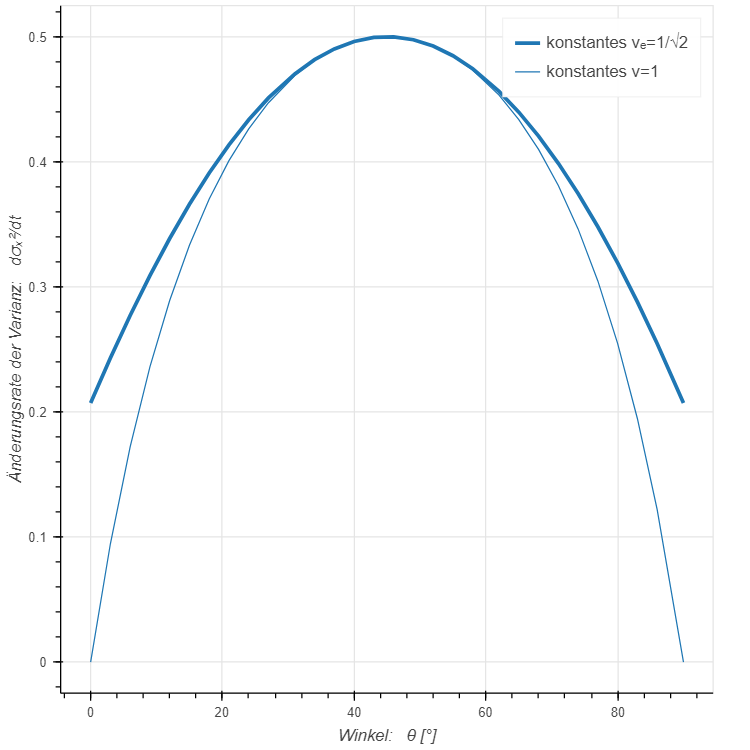
\includegraphics[width=8cm]{varianz-winkel.png}
\caption{$\frac{\operatorname{d}\sigma_x^2}{\operatorname{d}t}$ in Abhängigkeit von $\theta$}
\label{fig_variance_angle}
\end{figure}

\subsection{Literatur}

\end{document}
